\section{Important Concepts}
\label{sec:concepts}

This section describes the definitions of the important concepts
regarding our representations on API usages.

%\begin{figure}[t] %[!htp]
%	\centering
%	\includegraphics[width=0.9\linewidth]{aug-example}
%        \vspace{-3pt}
%	\caption{An API Usage and its API-Usage Graph}
%	\label{fig:aug}
%\end{figure}

\begin{Definition}[API elements]
An API element is either a class, a method, or a field that is
provided in a library to enable the accesses to the library's
functions via a variable declaration with a certain class, a method
call to an API method, or a field access to an API field.
\end{Definition}

For example, in Fig.~\ref{fig:example1}, line 2, \code{AuthState} is
an API class, which is a declared type for the variable
\code{authstate}. At line 3, \code{isPreemptive} is an API
method, which is called on the variable \code{authstate}.

\begin{Definition}[API Usage]
An API usage consists of a set of API elements and control structures
(i.e., conditions and repetitions), together with other program
elements (e.g., variables, parameters, etc.) in specific combinations
and orders to perform a programming task.
\end{Definition}

In Fig.~\ref{fig:example1}, lines 2-5 show an API usage consisting of
1) a variable \code{authstate}, 2) its declared class
\code{AuthState}, 3) a method call to \code{getHostAuthState()} on the
variable \code{method}, 4) a method call to \code{isPreemptive()}, 5)
a conditional structure with \code{if}, 6) a method call to
\code{invalidate()}, and 6) a method call to
\code{setAuthRequested(...)}.

To represent an API usage, we adopt a graph-based representation
called {\em API-Usage Graphs (AUGs)}~\cite{msr19}.

\begin{Definition}[API Usage Graph (AUG)~\cite{msr19}]
AUG is a directed, connected graph with labelled nodes and
edges. Nodes represent data entities (variables, values), and actions,
(method calls or operators). Edges represent the API usage
relations among the entities and actions represented by nodes.
\end{Definition}

The usage relations are defined as follows.

\begin{Definition}[API Usage Relation]
  In an API usage, there exist the API usage relations among the API
  elements and relevant program elements. The API usage relations
  include the following ones: {\bf receiver, parameter, definition,
    order, condition, synchronize, throw, handle}, and {\bf data and
    control dependencies} among the API and program elements.
\end{Definition}

Let us use the term {\em action nodes} to refer to method calls, field
accesses, or operators, and the term {\em data nodes} to represent
objects, values, and literals that appear in API usages. A {\em
  receiver} relation exists between a variable and a method call. A
{\em parameter} relation connects an argument to be used as a
parameter of an action. A {\em definition} relation exists between a
constructor or method call that creates or returns a value or object
to the respective variable. An {\em order} relation connects two
actions on operating on the same receiver or parameter. A {\em
  condition} relation connects an action whose result controls
branching to an action being controlled. A {\em synchronize} relation
connects a variable that the program obtains a lock on to an action
executed under that lock. A {\em throw} relation connects an action
that may throw an exception to a data node representing that exception
object. A {\em handle} relation connects from a \code{catch} action to
an action in a respective exception handling block.

We expect to leverage API usage relations among API elements
and relevant program entities for misuse detection.

\begin{figure}[t] %[!htp]
	\centering
	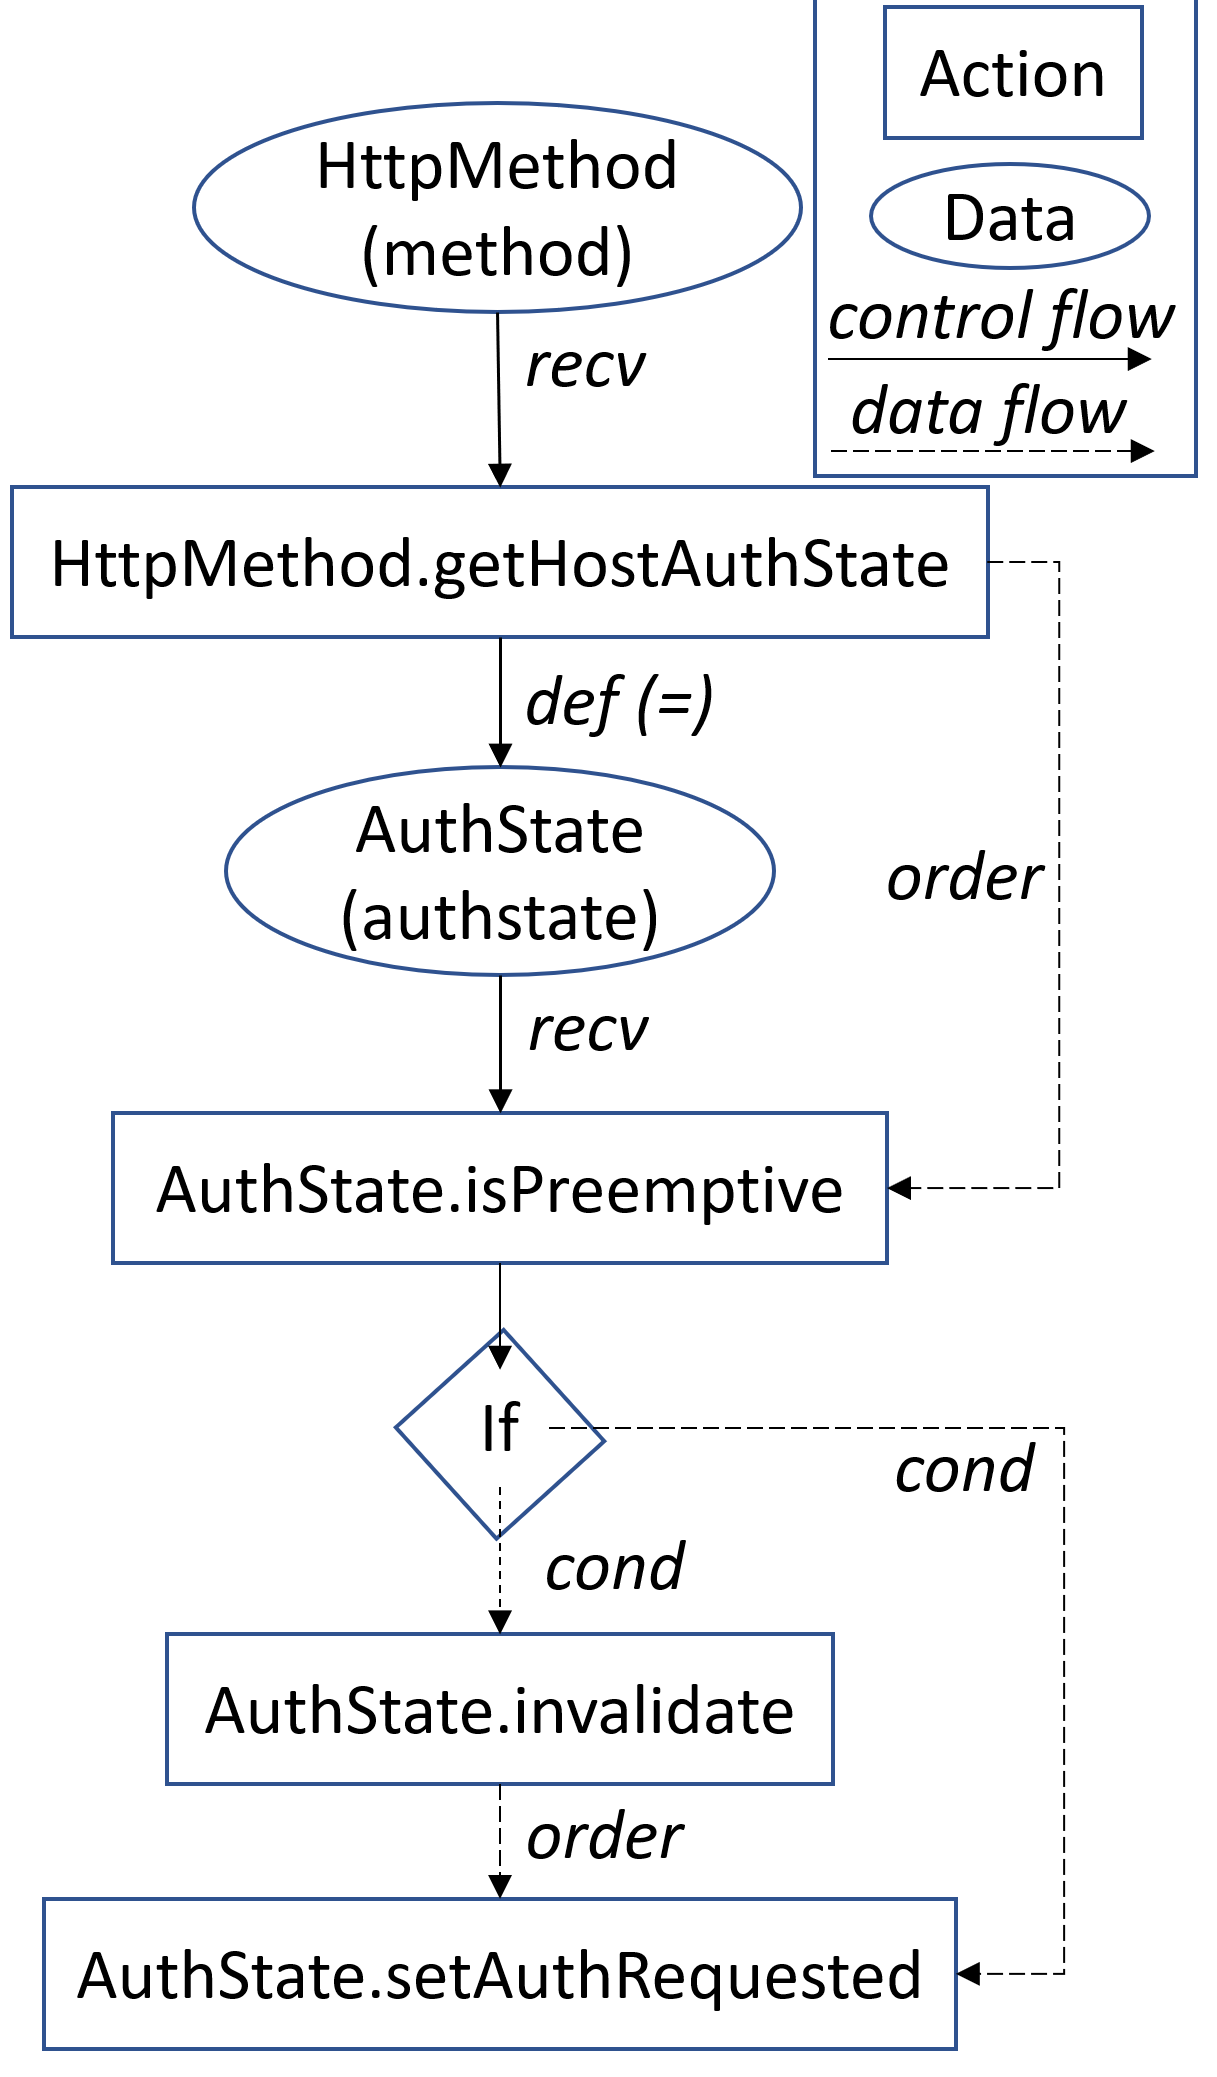
\includegraphics[width=1.8in]{aug}
        \vspace{-3pt}
	\caption{API-Usage Graph for Fig.~\ref{fig:example1}}
	\label{fig:aug}
\end{figure}

Fig.~\ref{fig:aug} shows the AUG of the code in
Fig.~\ref{fig:example1}.  The action nodes are displayed in the
rectangles and the data nodes in the oval shapes. The action nodes
represent method calls \code{Http\-Method\-.get\-Host\-Auth\-State},
\code{Auth\-State\-.isPre\-emptive}, \code{Auth\-State.\-invalidate},
\code{Auth\-State\-.set\-Auth\-Requested}. If the types are available,
they will be resolved. However, in the figure, only the simple name is
shown for clarity. The data nodes represent the variable \code{method}
with the type \code{Http\-Method}, and the variable \code{authstate}
with the type \code{Auth\-State}. The condition node \code{if}
represents the \code{if} structure at line 3 of
Fig.~\ref{fig:example1}.

There is a \code{recv} edge from \code{HttpMethod} to
\code{get\-Host\-Auth\-State} (line 2) and another \code{recv} edge
from \code{Auth\-State} to \code{isPre\-emptive} (line 3). There is a
\code{def} edge from \code{get\-Host\-Auth\-State} to
\code{Auth\-State} because the assignment statement at line 2 to
define the variable \code{auth\-state}. An \code{order} edge exists
between \code{get\-Host\-Auth\-State} and \code{is\-Pre\-emptive}
because the former needs to be executed before the latter. Similar
treatment is applied for \code{invalidate} and
\code{set\-Auth\-Requested}. Because the \code{if} node represents the
branching point in the condition structure, \code{isPre\-emptive} is
executed before \code{if}. Finally, there are two \code{cond} edges
from \code{if} to either \code{invalidate} and
\code{set\-Auth\-Requested} due to the control flows from the
branching point to either branch.

%(\code{init}), method calls, field accesses, and operators. If the
%types are available, they will be resolved. However, in the figure,
%only the simple name is shown for clarity. The relational operators
%are also encoded as actions to capture conditions. The data nodes
%represent objects, values, and literals in an API usage. AUG encodes
%data entities as nodes to make explicit the data dependencies between
%actions, such as multiple calls on the same object to ensure we have a
%connected subgraph with all data-dependent parts of a usage. The usage
%relations are shown with their labels. {\em Order} edges are not
%shown for clarity. The AUG building algorithm is explained in~\cite{msr19}.
